\documentclass[11pt,a4paper]{article}

\usepackage[margin=1in]{geometry}
\usepackage{titlesec}
\usepackage[table]{xcolor}
\usepackage{array}
\usepackage{graphicx}
\usepackage{longtable}
\usepackage{tabularx}
\usepackage{enumitem}
\usepackage{fancyhdr}
\usepackage{hyperref}
\usepackage{textcomp}
\usepackage{tikz}
\usetikzlibrary{positioning, arrows.meta}

\definecolor{headingblue}{RGB}{31,73,125}
\definecolor{tableblue}{RGB}{47,117,181}
\definecolor{lightbox}{RGB}{234,241,247}

\titleformat{\section}
  {\large\bfseries\color{headingblue}}
  {\thesection}{0.6em}{}
\titleformat{\subsection}
  {\normalsize\bfseries\color{headingblue}}
  {\thesubsection}{0.6em}{}

\pagestyle{fancy}
\fancyhf{}
\fancyhead[L]{\small DSA with C++ \\ Team ID: DSCPP-III-2026-T272}
\fancyfoot[R]{\small Page \thepage}
\renewcommand{\headrulewidth}{0pt}
\setlength{\headheight}{28pt}

\hypersetup{
  colorlinks=true,
  urlcolor=headingblue,
  linkcolor=headingblue
}

\begin{document}

\begin{center}
  {\Huge\bfseries\color{headingblue} PROJECT PROPOSAL}\\[0.3em]
  {\large\itshape Data Structures \& Algorithms with C++}
\end{center}

\vspace{1em}

\section*{Project and Team Information}
\vspace{-0.5em}
\noindent\rule{\linewidth}{0.8pt}

\subsection*{Project Title}
\begin{center}
\fcolorbox{black}{lightbox}{
  \parbox{0.9\linewidth}{\centering \bfseries\itshape Smart Expense Splitter}
}
\end{center}

\subsection*{Student / Team Information}

\begin{center}
\renewcommand{\arraystretch}{1.6}
\begin{tabularx}{\linewidth}{|>{\bfseries}l|X|c|}
\hline
\rowcolor{tableblue}
\textcolor{white}{Team Name} & \textcolor{white}{Avengers} & \\
\hline
Team Lead &
\textbf{Tanmay Kumar} \newline
2510370439 \newline
2510370439@geu.ac.in &
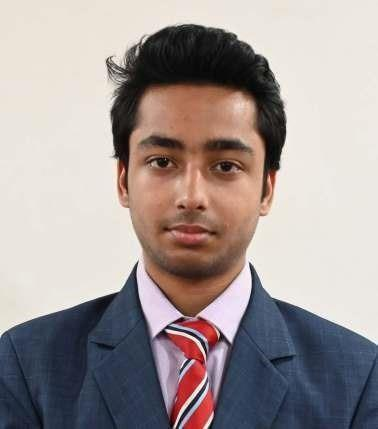
\includegraphics[width=2.2cm]{figs/tanmay.jpg} \\
\hline
Team Member 2 &
\textbf{Hemang Sethi} \newline
2510370341 \newline
2510370341@geu.ac.in &

\includegraphics[width=2.2cm]{figs/hemang.jpg} \\
\hline
Team Member 3 &
\textbf{Sparsh Saxena} \newline
2510370313 \newline
2510370313@geu.ac.in &
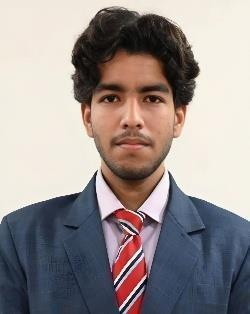
\includegraphics[width=2.2cm]{figs/sparsh.jpg} \\
\hline
\end{tabularx}
\end{center}

\clearpage

\section*{Proposal Description}
\noindent\rule{\linewidth}{0.8pt}

\subsection*{Motivation}

Settling up is usually the most annoying part. Say one person covers Rs.\,1{,}000 for dinner, someone else puts in Rs.\,500 for a cab, and others pay small amounts here and there. Trying to work out the bare minimum transfers by hand gets confusing fast. If people are traveling and spending in different currencies, nobody wants to sit and do manual conversions on every bill.

Smart Expense Splitter takes care of this math for you. Once you add your group and log the expenses, it tracks running balances and shows the direct payments needed so everyone gets squared away without the headache.

On the technical side, we are building this in C++ with an Object-Oriented setup, splitting responsibilities across \texttt{User}, \texttt{Group}, and \texttt{Transaction} classes. We are using operator overloading so balance calculations and settlements read naturally in code, along with templates so currency values and floating-point math stay flexible without having to rewrite functions.

\subsection*{Project Goals and Milestones}

Our main goal is to cut down on messy manual calculations and keep group balances clear so there is no confusion about who paid what.

\medskip
\noindent\textbf{The major goals of the project are to:}
\begin{itemize}[leftmargin=1.5em]
  \item Structure the C++ code around core classes like \texttt{User}, \texttt{Group}, and \texttt{Transaction}.
  \item Let users set up groups and split bills across different sets of members.
  \item Automatically track each person's share, what they paid, and their current net balance.
  \item Use operator overloading to keep balance updates and settlements clean and expressive.
  \item Use C++ templates to handle different currency types and precision levels without duplicate code.
  \item Provide an efficient method for settling balances between group members with fewer transactions.
  \item Create a simple interface that makes the project easy to understand and demonstrate in real-life scenarios.
\end{itemize}

\subsection*{Project Milestones}

\begin{center}
\renewcommand{\arraystretch}{1.4}
\begin{tabularx}{\linewidth}{|c|>{\bfseries}l|X|}
\hline
\rowcolor{tableblue}
\textcolor{white}{\#} & \textcolor{white}{Milestone} & \textcolor{white}{Description} \\
\hline
1 & Requirement Analysis & Identify common expense-sharing situations and finalize the features, inputs, and expected outputs. \\
\hline
2 & System Design & Design the class structure and relationships between \texttt{User}, \texttt{Group}, and \texttt{Transaction}. Plan the balance calculation and settlement logic. \\
\hline
3 & Core Implementation & Implement the basic C++ classes, constructors, data members, and functions for managing users, groups, and expenses. \\
\hline
4 & Advanced OOP Features & Implement operator overloading for balance operations and templates for currency handling. \\
\hline
5 & Testing and Debugging & Test the application with different group sizes, expenses, and currencies to identify and correct errors. \\
\hline
6 & Final Demonstration & Integrate all features, prepare sample real-life scenarios, document the project, and demonstrate the completed expense-splitting system. \\
\hline
\end{tabularx}
\end{center}

\subsection*{Project Approach}

The Smart Expense Splitter will be implemented using the concept of C++ to demonstrate the difference between procedural and object-oriented approaches. The application will allow users to create groups, record shared expenses, calculate individual shares, maintain balances, and settle payments efficiently.

In the C++ implementation, the same functionality will be developed using Object-Oriented Programming. Separate classes such as ``User'', ``Group'', and ``Transaction'' will provide better organization and encapsulation. Vectors will be used for dynamic storage. Operator overloading will be implemented for balance calculations and comparisons, while templates will provide reusable support for different numeric types and currencies.

\subsection*{Algorithms Used}

\begin{enumerate}[leftmargin=1.8em]
  \item \textbf{User/Group Management Algorithm:} Add, search, display, and manage group members.
  \item \textbf{Expense Recording Algorithm:} Store the payer, amount, participants, and currency for every transaction.
  \item \textbf{Expense Splitting Algorithm:} Divide the expense among selected members and calculate each person's share.
  \item \textbf{Balance Calculation Algorithm:} Balance = Amount Paid $-$ Amount Owed
  \item \textbf{Debt Settlement Algorithm:} Separate members into creditors and debtors and match them to determine who should pay whom.
  \item \textbf{Transaction Minimization Algorithm:} Continue matching debtors with creditors until all balances become zero or sufficiently close to zero.
  \item \textbf{Currency Handling:} Store currency information and use conversion logic where required. Templates in C++ will make the numerical implementation reusable.
\end{enumerate}

\subsection*{Technologies and Concepts}

\textbf{C++:} Classes and objects, encapsulation, constructors, vectors, inheritance where applicable, operator overloading, templates, and STL.

\textbf{Common:} Expense-splitting logic, balance calculation, debt settlement, searching, sorting, and file-based data storage.

The project will be tested using relatable scenarios such as hostel expenses, restaurant bills, group trips, and shared shopping, making it simple to demonstrate the C++ implementation.

\clearpage

\section*{System Architecture (High Level Diagram)}
\noindent\rule{\linewidth}{0.8pt}

\begin{center}
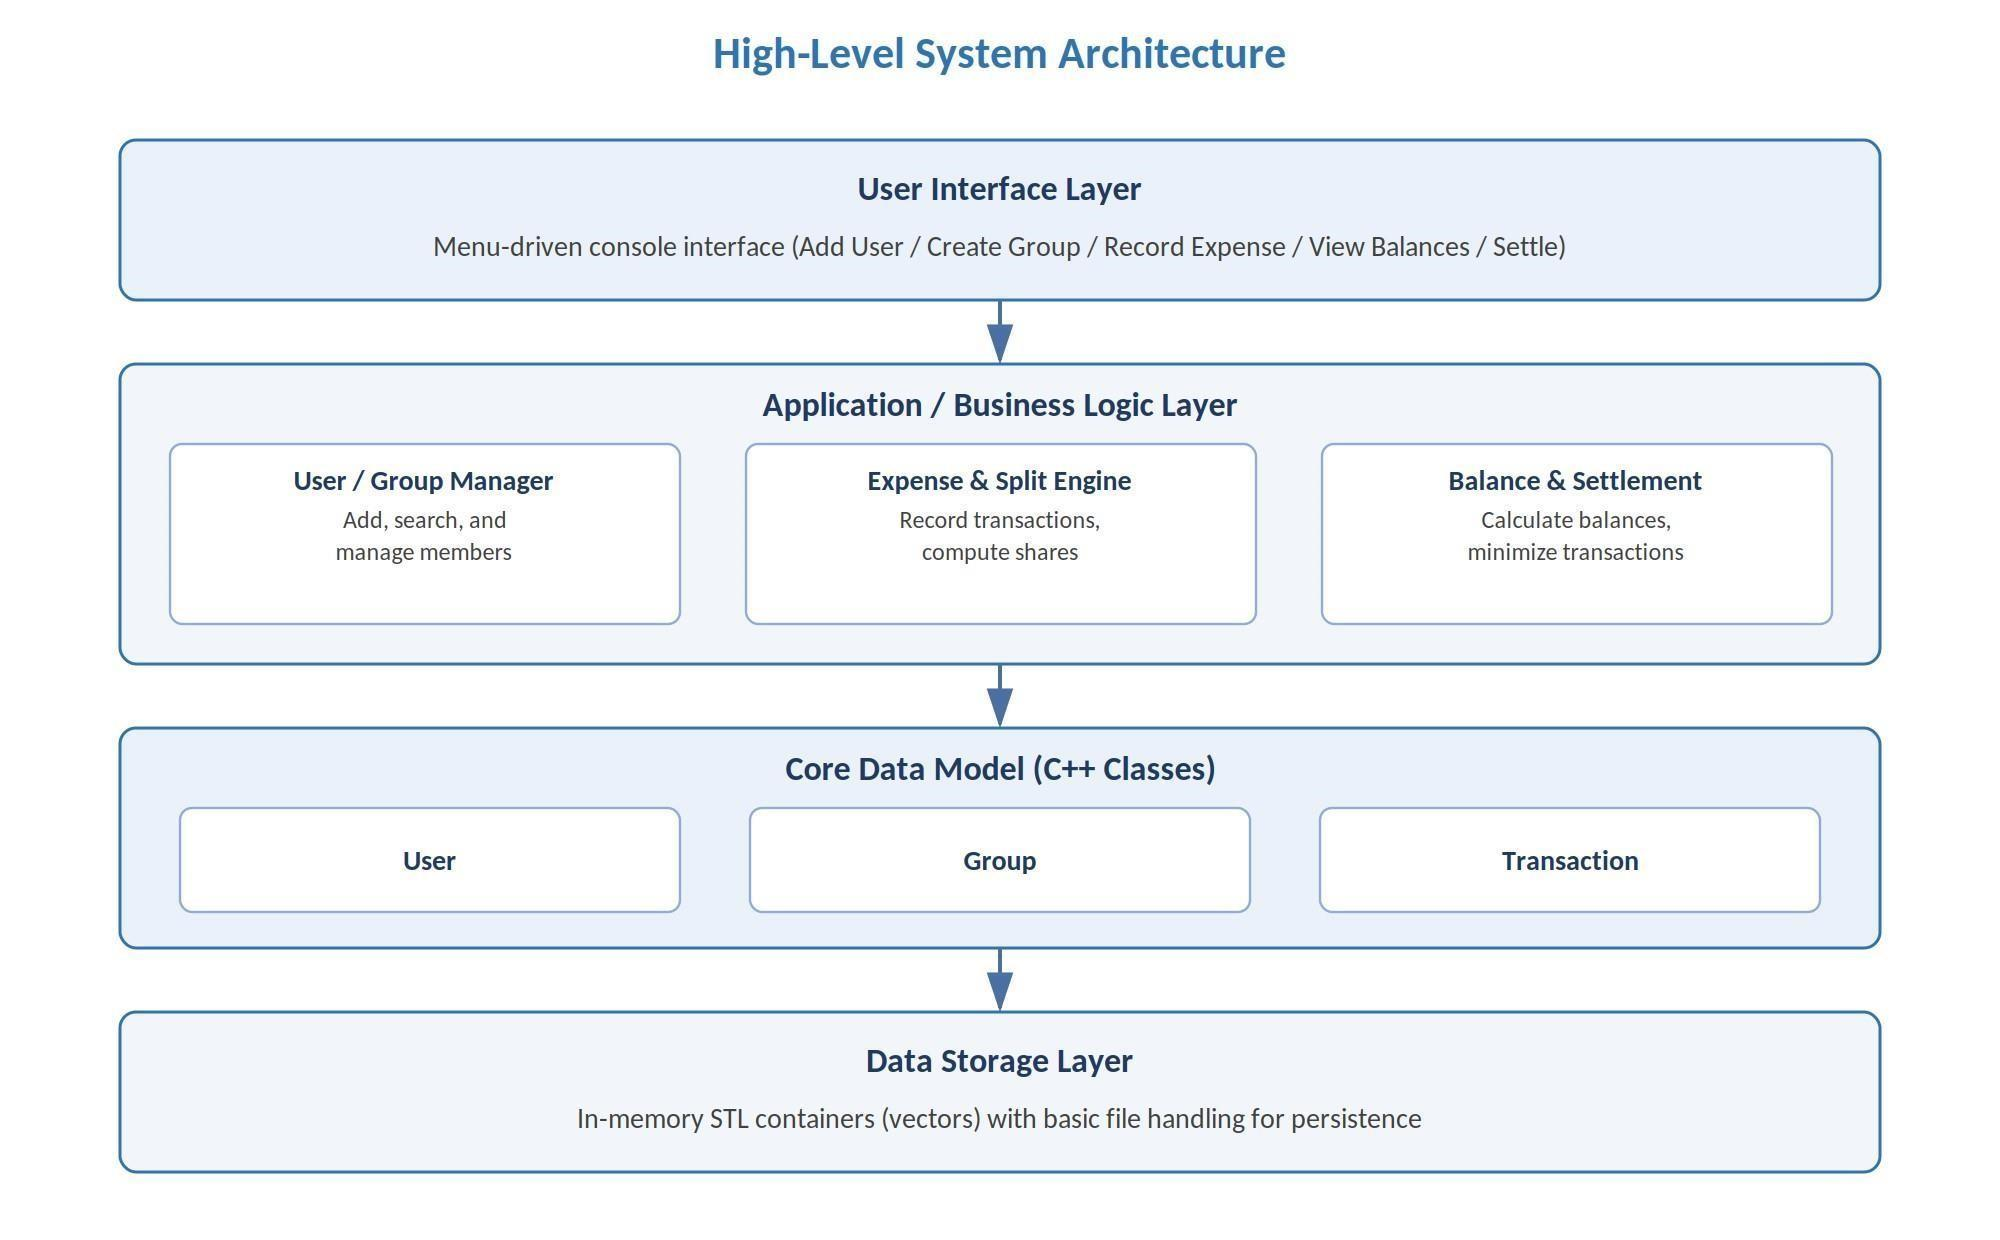
\includegraphics[width=0.95\linewidth]{figs/architecture.jpg}
\end{center}

\subsection*{Project Outcome / Deliverables}

The Smart Expense Splitter will provide a simple and efficient solution for managing shared expenses among friends, roommates, classmates, and travel groups. The project will automatically calculate individual contributions, determine outstanding balances, and simplify the process of settling debts between members. This will reduce the need for manual calculations and minimize errors, confusion, and disputes related to shared payments.

The project will also demonstrate the practical application of Data Structures, Algorithms, and C++ programming concepts. The C++ implementation will demonstrate Object-Oriented Programming, operator overloading, templates, and STL.

The system will be helpful in real-life situations such as hostel expenses, group trips, restaurant bills, rent sharing, and shopping. It will provide a clear record of who paid, who owes money, and the amount to be settled. Overall, the project will combine practical financial management with programming concepts to create a relatable, useful, and easy-to-demonstrate application.

\subsection*{Assumptions}

The project assumes that all users involved in an expense are already registered in the respective group and that valid information is provided while entering transactions. Expenses are assumed to be divided equally among the selected members, with one person initially paying the complete amount. Currency conversion, if required, will use predefined exchange rates rather than live rates. The system will not consider interest, penalties, or additional charges. User IDs are assumed to be unique for accurate transaction tracking. Data may be stored during program execution or through basic file handling.

\subsection*{References}

\begin{itemize}[leftmargin=1.5em]
  \item cppreference.com. (n.d.). \textit{C}. Retrieved September 1, 2026, from \url{https://en.cppreference.com/w/c}
  \item cppreference.com. (n.d.). \textit{C++}. Retrieved September 1, 2026, from \url{https://en.cppreference.com/w/cpp}
  \item cppreference.com. (n.d.). \textit{C++ standard library}. Retrieved September 1, 2026, from \url{https://en.cppreference.com/w/cpp/standard_library}
  \item cppreference.com. (n.d.). \textit{C++ reference book list}. Retrieved September 1, 2026, from \url{https://en.cppreference.com/w/cpp/books}
  \item Graphic Era University, Department of Computer Science and Engineering. (2026). \textit{Project-based learning (PBL) course material: Data Structures \& Algorithms with C/C++} [Unpublished course handout].
\end{itemize}

\end{document}
